\documentclass{article}

\usepackage{pdfsync}
\usepackage{natbib}
\usepackage{hyperref}

% dot graphs
\usepackage{dot2texi}
\usepackage{tikz}
\usetikzlibrary{shapes,arrows}

\begin{document}
	\author{Robin Deits\\ rdeits@csail.mit.edu}
	\title{6.375 Proposal: Adaptive PIV}
	\date{\today}
	\maketitle

	\section{Background: PIV} % (fold)
	\label{sec:background}
	Particle Image Velocimetry (PIV) is an optical approach to measuring the flow field of a fluid, and has been used in the study of combustion, water flow, robotics, and many other fields. It involves seeding a fluid with tracking particles and using a laser or other planar lighting system to capture sequential images of the particle positions in a single thin 2D slice of the fluid. By comparing the change in position of groups of particles between the subsequent frames, a measurement of the local flow vector can be computed for each region of the fluid. This process of determining the movement of each section of the image is extremely time-consuming in a sequential programming system, but can be readily parallelized to significantly improve performance \citep{Yu:2006tb}

	Each PIV computation is performed on a pair of sequential images. Computation of the fluid flow begins by dividing the image up into small windows of, for example, 64px on a side. A small window size helps ensure that all of the particles within the window move with the same velocity between the two frames. For each window, we extract the subimage corresponding to that window from the first image in the pair. We will call this subimage $A$. We then extract a set of subimages $B_{\Delta x,  \Delta y}$ by shifting the original window in two dimensions and extracting the corresponding subimages from the second image in the pair. We can then perform a cross-correlation between $A$ and each $B_{i, j}$ and determine the shift in $x$ and $y$ which maximizes the correlation. This gives the most likely location of the particles from window $A$ in the second frame, and thus indicates the movement of that section of the fluid between the frames.
	% section background (end)

	\section{Adaptive PIV} % (fold)
	\label{sec:adaptive_piv}
	Standard PIV algorithms involve an even spatial distribution of interrogation windows $A$ with a fixed window size and some fixed overlap, such as 64\,px windows beginning every 16\,px. However, in order to achieve sufficient accuracy in busy fluid flows, it can be necessary to choose very small windows or very high degrees of overlap, which increases the computational demands by requiring far more cross-correlation computations. 	Theunissen et al. proposed a method for improving the performance of PIV in sub-optimial conditions, called Adaptive PIV \citep{Theunissen:2009cr}. Their method uses information about the current density of seeding particles and the prior estimate of the velocity field to update the size and spatial frequency of the interrogation windows $A$. This has the effect of increasing the number of data points in the busiest (highest particle density and highest velocity) parts of the fluid and reducing the number of samples in the most stable areas of the fluid, which can improve the amount of relevant data collected per computational unit. 

	In this project, I will focus on implementing Adaptive PIV on an FPGA to improve computational performance, with the ultimate goal of allowing accurate real-time fluid tracking. I will be expanding on prior work implementing a standard PIV algorithm on an FPGA \citep{Yu:2006tb}. I will also be using a recent \textsc{Matlab} implementation of the Adaptive PIV algorithm by Samvaran Sharma of the Robot Locomotion Group at MIT CSAIL as the reference code for my implementation. 

	The primary benefit of this project should be the parallelization and speedup of the Adaptive PIV algorithm. In order to achieve the desired image size and accuracy, Sharma's current software requires approximately 2.5 seconds per pair of frames, which makes real-time analysis of the fluid flow impossible. In contrast, Yu et al. were able to compute 15 image pairs per second using their FPGA implementation. My goal will be to achieve this result with the added benefits of the adaptive algorithm's focus on the most important areas of the fluid flow.
	% section adaptive_piv (end)

	\section{Implementation}
	I will divide the implementation of the PIV system up into the high-level logic, which will be performed in \textsc{Matlab}, and the computationally intensive and parallelizable cross-correlation which will be performed on the FPGA. This division is shown in Figure~\ref{fig:system}. The host machine will read image pairs from disk (simulating live capture from a camera system), then convert them to 8-bit grayscale. These image pairs will be transmitted over SCEMI to the FPGA, which will store both images in DRAM. The host machine will then select a series of interrogation windows. The exact method of selection will depend on whether we are performing normal or adaptive PIV. The host will transmit the coordinates of the interrogation windows to the DUT. The FPGA will then extract the actual image data for each window, perform the cross-correlation, and locate the peak in the cross-correlation value signifying the displacement of the particles in the window. The FPGA will then send the displacement back to the host. 

	\subsection{Module: Window Store}
	The FPGA implementation will include two Window Store instances. Each Window Store will handle extracting windows from the source image and providing the individual pixel data for cross-correlation. The Window Store will need to support the following operations: 

	\begin{enumerate}
		\item loadWindow(x, y): extract an image window from the location (x, y) and store it in slice registers or in block RAM (to be determined).
		\item getNextPixel(): return the value of the next pixel needed for cross-correlation computation. Since the order in which pixel values are accessed is fixed, this function needs no input.
	\end{enumerate}


\begin{figure}[htbp]
\makebox[\textwidth][c]{
	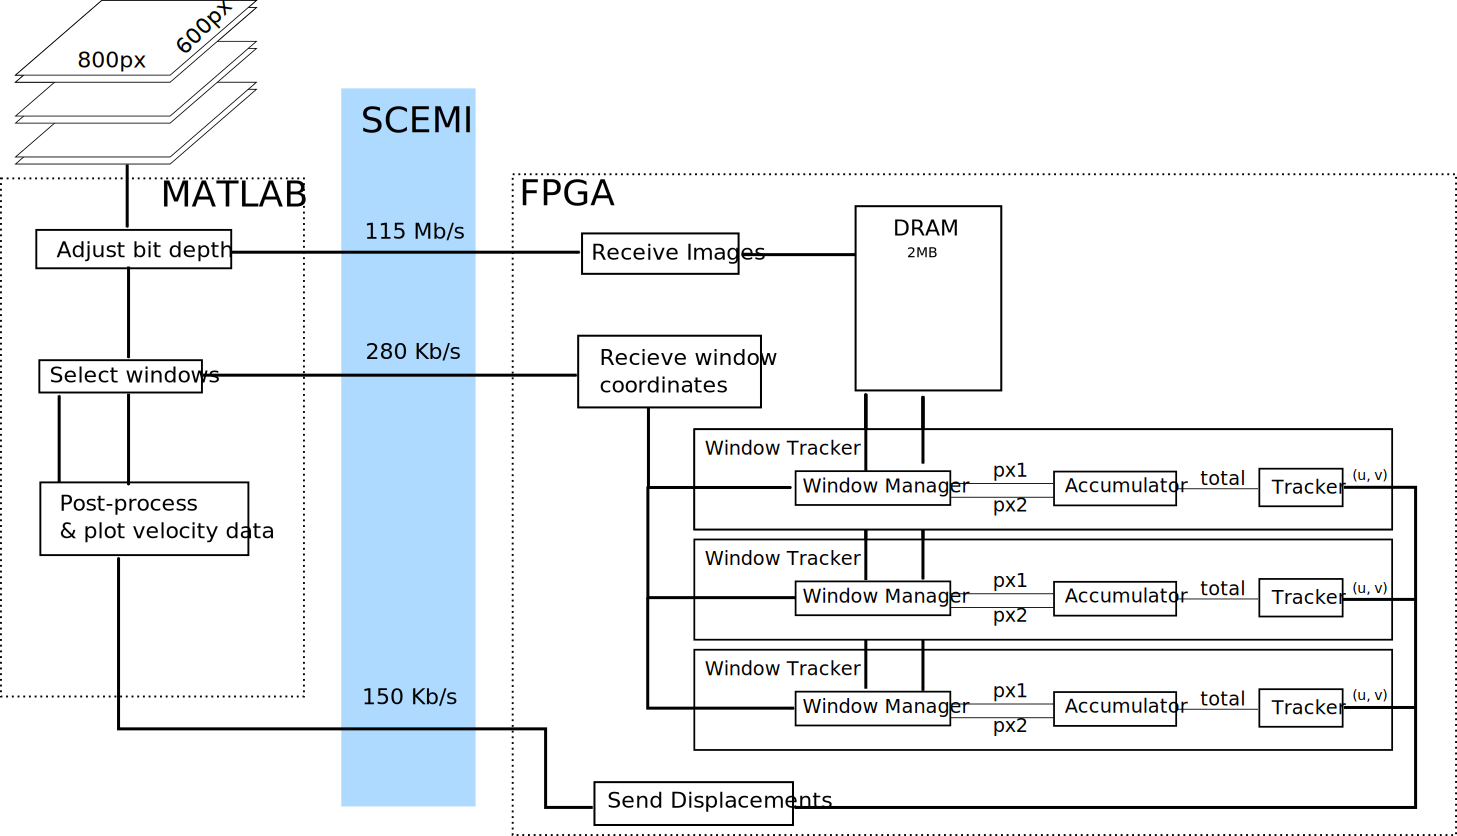
\includegraphics[width=1.2\textwidth]{system_diagram.pdf}}
	\caption{The system diagram for the Adaptive PIV implementation on the FPGA. High-level logic relating to the particular PIV implementation is performed in \textsc{Matlab}, and the cross-correlation is performed on the FPGA.}
	\label{fig:system}
\end{figure}



	\bibliographystyle{plain}
	\bibliography{refs}
\end{document}